\chapter{Grundlagen}



% Wortherkunft ====================================
\section{Wortherkunft}
\label{sec:wortherkunft}

\begin{description}
\item[Bus] „omnibus“ lat. „für alle“
\item[hier:] Kommunikationsmedium „für alle“
\item[klass. „shared medium“:] Was einer der Teilnehmer auf dem Medium sendet, hören (potentiell) alle Teilnehmer gleichzeitig mit.
\end{description}
% =================================================



% Topologien ======================================
\section{Topologien von „Computernetzen“}
\label{sec:topologien}

\subsubsection{Stern}
\begin{figure}[htbp]
  \centering
  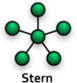
\includegraphics[scale=1]{Stern-Topologie.png}
  \caption{Stern-Topologie}
\end{figure}
Es gibt einen zentralen „Sternverteiler“ in der Mitte und dedizierte Leitungen von diesem zu jedem der Teilnehmer. Üblicherweise ist der Sternverteiler \underline{nicht} auch ein „normaler Teilnehmer“.\\

\subsubsection{Ring}
\begin{figure}[htbp]
  \centering
  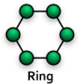
\includegraphics[scale=1]{Ring-Topologie.png}
  \caption{Ring-Topologie}
\end{figure}
Jeder Teilnehmer hat genau einen Vorgänger und einen Nachfolger, mit denen er jeweils verbunden ist.

\subsubsection{Bus}
\begin{figure}[htbp]
  \centering
  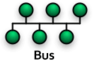
\includegraphics[scale=1]{Bus-Topologie.png}
  \caption{Bus-Topologie}
\end{figure}
Es gibt lediglich eine „Leitung“ als „shared medium“, mit welchem jeder Teilnehmer über eine „Stichleitung“ verbunden ist.

\subsubsection{Maschennetz}
\begin{figure}[htbp]
  \centering
  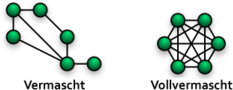
\includegraphics[scale=1]{Vermascht-Topologie.png}
  \caption{Maschen-Topologie}
\end{figure}
Jeder Teilnehmer hat zu beliebig vielen anderen Teilnehmern jeweils eine dedizierte Verbindung. Beim Spezialfall Vollvermascht hat jeder Teilnhemer eine Verbindung zu demem anderen Teilnehmer.

\subsubsection{Baum}
\begin{figure}[htbp]
  \centering
  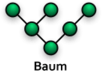
\includegraphics[scale=1]{Baum-Topologie.png}
  \caption{Baum-Topologie}
\end{figure}
Die Baumtopologie ist eine hierarchische Topologie. Ausgehend von einem „Wurzel Teilnehmer“ gibt es jeweils ein oder mehrere Verbindungen zu Teilnehmern der nächsten Hierarchieebene.

\subsubsection{Linie}
\begin{figure}[htbp]
  \centering
  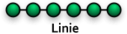
\includegraphics[scale=1]{Linie-Topologie.png}
  \caption{Linien-Topologie}
\end{figure}
Jeder Teilnehmer ist mit maximal zwei Teilnehmern verbunden. Es gibt einen Anfang und ein Ende.
% =================================================



% Bustopologie ====================================
\section{Verwenden alle „Bussysteme“ eine Bustopologie?}
\begin{table}[h]
\centering
\begin{tabular}{c|c}
\textbf{Bustopologie} & \textbf{Bustopologie} \\ 
\hline 
Ethernet in BNC-Verkabelung & USB: Baum \\ 
\hline 
ProfiBus & MOST: Ring \\ 
\hline 
WLAN & Ethernet in TP-Verkabelung: Baum \\ 
\hline
IDE (P-Data) & (S-ATA)\\
\hline
PCI & (PCI-Express)\\
\hline
SCSI & (SAS (Seriell Attached SCSI))\\
\hline
 & Firewire: vermaschtes Netz\\
 & mit Einschränkungen
\end{tabular}
\caption{Einordnung von Technologien in Bussysteme}
\label{tab:bussystem_or_not}
\end{table} 
Viele der heutigen „Bussysteme“ sind physikalisch keine \underline{Busse}, sondern nur noch logisch/protokolltechnisch auf einer höheren Ebene.
% =================================================



% Spezielle Aufgaben von Bussystemen ==============
\section{Spezielle Aufgaben von Bussystemen}
\label{sec:spezielle_Aufgaben_Bussysteme}
Speziell bei Bussystemen zu lösende Aufgaben:
\begin{itemize}
\item Medienzugriff
\item Adressierung
\end{itemize}
% =================================================